% main.tex — ACL 2023 format
% viscode_shared_subspace_probe
% Compile: pdflatex main && bibtex main && pdflatex main && pdflatex main

\documentclass[11pt]{article}

% --- ACL 2023 style ---
% If acl.sty is available, use it; otherwise fall back to a compatible setup.
% Uncomment the appropriate line:
\usepackage[review]{acl}    % anonymous submission mode
% \usepackage{acl}           % camera-ready (de-anonymized)

% Fix line numbers in two-column mode: put numbers on outer margin of each column.
% acl.sty loads lineno with [switch] which alternates by page parity, not column.
% Override \makeLineNumber after acl.sty's \AtBeginDocument{\linenumbers} fires.
\makeatletter
\AtBeginDocument{%
  \def\makeLineNumber{%
    \if@firstcolumn
      \makeLineNumberLeft
    \else
      \makeLineNumberRight
    \fi
  }%
}
\makeatother
\setlength{\linenumbersep}{5pt}

% --- Core packages ---
\usepackage{times}
\usepackage{latexsym}
\usepackage[T1]{fontenc}
\usepackage[utf8]{inputenc}
\usepackage{microtype}
% \usepackage{inconsolata}  % optional monospace font

% --- Math & tables ---
\usepackage{amsmath}
\usepackage{amssymb}
\usepackage{booktabs}
\usepackage{multirow}

% --- Figures ---
\usepackage{graphicx}
\graphicspath{{figures/}}
\usepackage{subcaption}

% --- Links ---
% hyperref is loaded by acl.sty; do not reload
\usepackage{url}

% --- Misc ---
% xcolor is loaded by acl.sty; do not reload
\usepackage{enumitem}
\usepackage{pifont}    % \ding{51} checkmark, \ding{55} cross
\usepackage{placeins}  % \FloatBarrier
\usepackage{algorithm}
\usepackage{algorithmic}

% --- Float tuning (prevent tables from drifting to end) ---
\renewcommand{\topfraction}{0.9}
\renewcommand{\bottomfraction}{0.8}
\renewcommand{\textfraction}{0.1}
\renewcommand{\floatpagefraction}{0.7}

% ============================================================
% Author block — anonymous for review
% ============================================================
\author{Anonymous}

\begin{document}

% Title, maketitle, and abstract (from title_abstract.tex)
% Title + Abstract
% viscode_shared_subspace_probe — D028/D029/D030 framing
% Generated: 2026-04-11

%% ============================================================
%% TITLE (11 words, no banned phrases)
%% ============================================================

\title{Cross-Format Representational Probing of Visual Code LLMs:\\A Training-Free Framework with a Qwen2.5 Case Study}

\maketitle

%% ============================================================
%% ABSTRACT (~230 words)
%% ============================================================

\begin{abstract}
% (1) Motivation
Large language models increasingly generate visual content through code---SVG, TikZ, Asymptote---yet their internal representations during this process remain unexplored.
Do models that handle multiple visual code formats develop format-agnostic representations, or are their hidden states predominantly format-specific?

% (2) Method
We introduce a training-free probing framework for measuring cross-format representational similarity in visual code LLMs.
The framework extracts hidden states via teacher-forcing, then applies linear Centered Kernel Alignment (CKA) with bootstrap confidence intervals, permutation null testing (5{,}000 permutations), and a Procrustes distance robustness check.

% (3) Findings — Qwen case study
Applying this framework to the Qwen2.5 family (Coder-7B-Instruct, base 7B, and VisCoder2-7B) across 252 semantically matched triples at 7 equidistant layers, we report five findings:
(1)~format identity is perfectly decodable at every layer (tokenization artifact);
(2)~cross-format CKA is statistically significant but weak ($2.8$--$3.0\times$ the permutation null, $p < 0.001$; bootstrap mean peak 0.154--0.187);
(3)~TikZ--Asymptote similarity systematically exceeds SVG--TikZ by $2$--$3\times$, following a token-overlap gradient (BPE Jaccard $\rho \approx 0.7$ at pair level) with layer-dependent modulation ($\rho = 0.57$ across 126 cells);
(4)~only Qwen2.5-base among six tested models exhibits a sharp final-layer CKA drop, which affects non-visual Python code ($-60\%$) more severely than visual code ($-37\%$), consistent with generic final-layer destabilization rather than visual-specific specialization;
(5)~visual-code supervised fine-tuning does not substantially alter cross-format structure.

% (3b) Cross-architecture generalizability
Cross-architecture validation on three additional models (Codestral-22B, StarCoder2-15B, DeepSeek-Coder-V2-Lite) spanning Mistral, BigCode, and MoE architectures confirms that the weak cross-format signal generalizes: all six models show $p < 0.001$ with obs/null ratios of $2.55$--$3.01\times$.
However, peak CKA depth is architecture-dependent (56--100\% depth), ranging from inverted-U profiles to broadly rising trajectories to bimodal patterns, ruling out a universal ``mid-layer peak'' characterization.

% (4) Significance
A pre-registered negative control (D060) formally fails: non-visual Python code yields 60--110\% of the visual cross-format CKA in magnitude at 20/21 evaluation cells, establishing that code-general structure---rather than visual-specific representations---dominates the measured alignment.
However, a code-naive ablation (Llama-3-8B) shows this failure mode is itself code-pretraining-specific: visual cross-format CKA persists without code pretraining (9/9 cells $p < 0.005$), while python--visual entanglement does not (7/9 cells $p > 0.10$).
We release the complete pipeline as a methodological template, emphasizing honest reporting of weak and ambiguous findings to advance rigorous representation analysis of code LLMs beyond behavioral evaluation.
\end{abstract}


% ============================================================
% Body sections
% ============================================================

% Introduction
% viscode_shared_subspace_probe — D028/D029/D030 framing
% Generated: 2026-04-11

\section{Introduction}
\label{sec:intro}

% P1: visual code generation booming, all behavioral eval
The generation of visual content through code is a rapidly growing capability of large language models.
Rather than producing raster images directly, these models synthesize programs in domain-specific formats---SVG for web graphics, TikZ for scientific figures, Asymptote for geometric illustrations---that compile into precise, scalable visual output.
Specialized systems such as VisCoder2 \cite{viscoder2}, LLM4SVG \cite{llm4svg2025}, and Chat2SVG \cite{chat2svg2025} have demonstrated increasingly sophisticated visual code generation, while general-purpose code LLMs like the Qwen2.5-Coder family \cite{qwen25coder} handle multiple such formats within a single model.
However, all existing evaluations of these models are \emph{purely behavioral}: models are judged by execution pass rates, VLM-judge scores, or CLIP similarity, with no analysis of what visual structure the models internally encode.

% P2: natural question
This leaves a fundamental question unanswered: \emph{do models that generate visual code in multiple formats develop format-agnostic internal representations of visual content, or are their hidden states predominantly format-specific?}
If different visual code formats converge to similar representations for semantically related visual programs, it would suggest that these models have abstracted visual semantics beyond surface syntax.
Conversely, if representations are entirely format-specific---as one might expect given the radically different tokenization of SVG (XML markup), TikZ (\LaTeX{} macros), and Asymptote (imperative C-like code)---it would imply that multi-format capability arises from disjoint pathways rather than shared computation.

% P3: our contribution
Addressing this question is methodologically non-trivial.
Unlike probing for discrete linguistic properties \cite{hewitt-manning-2019-structural, belinkov-2022-probing}, measuring representational similarity across output formats requires comparing hidden-state geometries for semantically related but syntactically distinct programs, with careful attention to small sample sizes and syntactic confounds.
In this work, we introduce a \textbf{training-free probing framework} for measuring cross-format representational similarity in visual code LLMs.
The framework operates entirely on cached hidden-state representations extracted via teacher-forcing, combining linear Centered Kernel Alignment (CKA; \citealt{kornblith2019similarity}) with bootstrap confidence intervals, permutation null testing, and a Procrustes distance robustness check.
We demonstrate this framework through a case study on the Qwen2.5 model family.

% P4-P5: compressed — findings already in Abstract
Our case study on three Qwen2.5-based 7B models finds statistically significant but weak cross-format CKA (${\sim}3\times$ the permutation null), lexically confounded at pair-level (BPE token Jaccard $\rho \approx 0.7$), with residual layer-dependent structure.
The observed similarity is of \textbf{uncertain origin}, and we present these results as a methodological template.
Our contributions are:

\begin{enumerate}
    \item \textbf{A training-free probing framework} for measuring cross-format representational similarity in LLMs, combining CKA with bootstrap confidence intervals, permutation null testing (5{,}000 permutations), power simulation, and Procrustes distance robustness check.

    \item \textbf{Five empirical findings} from a Qwen2.5 case study---the first representation-level analysis of multi-format visual code LLMs, including a pre-registered negative control that establishes the measured cross-format signal reflects code-general rather than visual-specific structure---demonstrating both the utility of the framework and the complexity of interpreting cross-format similarity signals.

    \item \textbf{An open-source analysis pipeline} covering data generation, hidden-state extraction, CKA computation, permutation testing, and visualization, designed for replication across model families beyond the single-family case study presented here.
\end{enumerate}



% Related Work
% viscode_shared_subspace_probe — D028 framing
% Generated: 2026-04-11

\section{Related Work}
\label{sec:related}

\paragraph{Visual code generation.}
Single-format specialists include LLM4SVG \cite{llm4svg2025} and Chat2SVG \cite{chat2svg2025} for SVG, DaTikZ \cite{datikz} and vTikZ \cite{vtikz2025} for TikZ, and VGBench \cite{vgbench2024} for multi-format evaluation.
VisCoder2 \cite{viscoder2} is a multi-format model trained on 12 visualization languages.
All prior work is \emph{purely behavioral}---evaluating execution pass rate or CLIP similarity---with no analysis of internal representations.
Our work fills this gap by examining hidden states during visual code processing.

\paragraph{Mechanistic interpretability of code LLMs.}
Probing and representation analysis have been extensively applied to natural language models \cite{belinkov-2022-probing}, but their extension to code LLMs is recent.
\citet{neuron-guided-2025} use neuron selectivity analysis and representational similarity analysis to identify concept layers shared across C++, Java, Python, Go, and JavaScript, finding that syntactic and semantic code concepts are encoded at consistent layers regardless of programming language.
\citet{sae-correctness-2025} train sparse autoencoders on code-LLM residual streams to discover directions predicting code correctness.
Our axis is orthogonal: where these works ask ``is \texttt{for-loop} represented the same way across Python and Go,'' we ask ``is \emph{red circle above blue square} represented the same way across SVG and TikZ.''
The probe targets are properties of the \emph{rendered image} (color, shape count, spatial layout), not of the code syntax.
To our knowledge, no prior work has examined image-grounded visual attributes in code-generation hidden states.

\paragraph{Representation probing and the linear representation hypothesis.}
Linear probing of neural network representations originated in NLP for analyzing syntactic and semantic structure \cite{hewitt-manning-2019-structural, conneau-etal-2018-what}.
The linear representation hypothesis \cite{park2024linear} posits that high-level concepts are encoded as linear directions in LLM residual streams, providing theoretical grounding for linear probe studies.
CKA (Centered Kernel Alignment) \cite{kornblith2019similarity} provides a representation-similarity metric invariant to invertible linear transformations, widely used for comparing representations across layers, models, and training stages.
We adopt the standard probing methodology but apply it to a novel domain: \textbf{cross-format representational similarity} in visual code LLMs, using CKA as the primary metric with Procrustes distance as the primary robustness check (PWCCA \cite{morcos2018pwcca} is included as a supplementary metric but limited by $n \ll d$; \S\ref{sec:robustness-pwcca}).

\paragraph{CKA: known limitations.}
While CKA is widely used, it has known limitations.
\citet{nguyen2021wide} show that CKA can be insensitive to functionally important differences between networks, particularly in wide architectures.
\citet{ding2021grounding} propose statistical grounding for representation similarity, noting that naive CKA lacks formal hypothesis testing.
\citet{tang2020similarity} survey functional and representational similarity measures, finding that linear CKA is sensitive to outliers in low-sample regimes.
We mitigate these concerns by pairing CKA with permutation null testing (providing formal $p$-values), bootstrap confidence intervals, and an independent Procrustes distance check.

\paragraph{Cross-format and cross-lingual transfer.}
The broader question of whether LLMs develop format-agnostic internal representations has been studied in multilingual NLP.
Cross-lingual probing shows that multilingual models learn partially shared representations across natural languages \cite{pires-etal-2019-multilingual, wu-dredze-2019-beto}, with shared structures emerging at intermediate layers.
In the code domain, \citet{neuron-guided-2025} demonstrate shared concept layers across programming languages.
Our work extends this line of inquiry to \textbf{visual code formats}: SVG, TikZ, and Asymptote share rendering semantics (2D vector graphics) but differ radically in syntax (XML markup, \LaTeX{} macros, imperative code), making them an ideal testbed for studying whether cross-format representational similarity reflects visual semantics or surface-level syntactic patterns.

\paragraph{Training-free analysis.}
Our framework requires no model training: we use off-the-shelf models, performing only inference and lightweight CPU-based linear probe fitting, in the tradition of training-free mechanistic analysis \cite{hewitt-manning-2019-structural, belinkov-2022-probing}.


% Methods
% viscode_shared_subspace_probe — D028 updated (no "shared subspace", no Step 4)
% Generated: 2026-04-11

\section{Method}
\label{sec:method}

\subsection{Overview}

We present a training-free framework for measuring cross-format representational similarity in visual code LLMs.
The design separates \textbf{behavioral generation} (Stage~A) from \textbf{representational probing} (Stage~B) using two independent tool stacks on two disjoint data pools, ensuring that generation ability and representation content are measured independently.
We demonstrate this framework through a case study on the Qwen2.5 model family.

\subsection{Models}

We study three 7B-parameter models spanning a generalist--specialist spectrum:

\begin{itemize}
    \item \textbf{Qwen2.5-Coder-7B-Instruct} \cite{qwen25coder} --- a code-specialized LLM instruction-tuned on broad programming tasks, serving as the primary model with demonstrated multi-format visual code capability.

    \item \textbf{Qwen2.5-7B} (base) --- the general-purpose pretrained model without code-specific instruction tuning, serving as a text-only control.
    Because Stage~B uses teacher-forcing (\S\ref{sec:stage-b}), base model hidden states reflect what the model \emph{encodes} when processing visual code tokens, regardless of whether it can \emph{generate} such code autonomously.

    \item \textbf{VisCoder2-7B} \cite{viscoder2} --- a Qwen2.5-Coder-7B-Instruct model further fine-tuned on VisCode-Multi-679K, a 679K-example multi-language visualization SFT corpus spanning 12 visual languages including SVG, TikZ, and Asymptote.
\end{itemize}

The headline analysis uses the first two models ($N{=}12$ cells: 2~models $\times$ 6~ordered format-pairs).
VisCoder2 is included in an auxiliary $N{=}18$ analysis reported as an \emph{exploratory view with known memorization floor}: its SFT training data overlaps with both our eval pool and probe pool sources (\S\ref{sec:contamination}), making its cells informative about contamination effects rather than clean cross-format similarity.

\subsection{Visual Code Formats}

We target three shape-drawing domain-specific languages that share common rendering semantics (2D vector graphics with color, position, and style attributes) while differing radically in syntax:

\begin{itemize}
    \item \textbf{SVG} --- XML-based markup with explicit coordinate attributes.
    \item \textbf{TikZ} --- \LaTeX{} macro language with relative/absolute positioning.
    \item \textbf{Asymptote} --- imperative C-like language with function calls.
\end{itemize}

This yields 3 unordered format-pairs (SVG--TikZ, SVG--Asy, TikZ--Asy) per model per layer.
Linear CKA is symmetric ($\text{CKA}(X,Y) = \text{CKA}(Y,X)$), so the headline $N{=}12$ statistic counts $3~\text{pairs} \times 2~\text{models (Coder, base)} \times 1 = 6$ independent CKA values per layer; including all 7 layers and 2 test statistics (CKA, Procrustes) yields 12 cells for the primary analysis.
VisCoder2 adds 6 cells to the auxiliary $N{=}18$ analysis.

\subsection{Stage A: Behavioral Generation}
\label{sec:stage-a}

Stage A establishes that the models under study can generate valid visual code, independent of Stage B's representational analysis.
We construct an eval pool of 200 captioned visual programs per format (600 total) from held-out test splits of VisPlotBench,\footnote{\url{https://huggingface.co/datasets/xingxm/VisPlotBench}} DaTikZ \cite{datikz}, and VisCode-Multi-679K \cite{viscoder2}.
Each caption is presented under 0-shot and 3-shot regimes, yielding 3{,}600 free generations evaluated by format validity and a hybrid content fidelity metric (CLIPScore \cite{clip} for high-SNR attributes; programmatic AST match for spatial attributes).
Generation parameters and results are in Table~\ref{tab:stage_a_summary} (Appendix).

\subsection{Stage B: Hidden-State Extraction}
\label{sec:stage-b}

\paragraph{Probe pool construction.}
The probe pool is constructed from \emph{training splits} of datasets disjoint from the eval pool: SVG from SVGX-Core-250k\footnote{\url{https://huggingface.co/datasets/xingxm/SVGX-Core-250k}} (${\sim}257$K), TikZ from DaTikZ v2 train \cite{datikz} (94{,}532), and Asymptote from VCM-Asy \cite{viscoder2} (22{,}539).

\paragraph{Cross-format semantic alignment.}
To enable meaningful cross-format comparison, we construct semantically matched triples (one caption per format describing a similar visual concept).
Captions are truncated to 50 tokens and embedded using \texttt{all-MiniLM-L6-v2} \cite{reimers2019sbert}.
A greedy matching algorithm retains triples where the minimum pairwise cosine similarity $\geq 0.70$.
This yields $N{=}252$ matched triples.
All 252 triples have minimum pairwise cosine $\geq 0.70$; CKA is therefore invariant to threshold choices in $[0.60, 0.70]$. At stricter thresholds ($0.75$, $N{=}51$; $0.80$, $N{=}6$), CKA increases but sample sizes enter severe $n \ll d$ regime (Table~\ref{tab:sbert_sensitivity}, Appendix).

\paragraph{Teacher-forced hidden-state extraction.}
For each (model, format, triple) combination, we construct a prompt from the caption and \emph{teacher-force} the corresponding reference code.
During the forward pass, we capture the residual stream at 7 equidistant layers $\{4, 8, 12, 16, 20, 24, 28\}$ and \textbf{mean-pool over code-token positions only} (masking caption, system, and chat-template tokens), producing one vector of dimension $d_\text{hidden} = 3{,}584$ per (model, layer, format, triple).

Teacher-forcing is the methodologically correct choice for representation probing \cite{hewitt-manning-2019-structural, belinkov-2022-probing}: free-generation hidden states confound generation ability with representation content.
By fixing the token sequence to a known-good reference, we isolate ``what the model encodes when it processes this visual concept in this format.''
This makes Qwen2.5-7B base a fair text-only control: it cannot generate valid visual code, but teacher-forcing reveals whether its representations nonetheless encode cross-format structure.

\subsection{Statistical Analysis}
\label{sec:analysis}

\paragraph{Centered Kernel Alignment (CKA).}
For each (model, layer, format-pair), we compute linear CKA \cite{kornblith2019similarity} between the two $252 \times 3584$ hidden-state matrices.
CKA measures representational alignment invariant to invertible linear transformations, yielding one similarity scalar per cell.

\paragraph{Format identity probe.}
We train a logistic regression classifier (\texttt{sklearn}, $C{=}1.0$, \texttt{max\_iter}${=}2000$) on the hidden-state vectors to predict format identity (3-way: SVG vs.\ TikZ vs.\ Asy).
This directly tests whether format-specific information is linearly decodable at each layer.

\paragraph{Bootstrap confidence intervals.}
We construct 95\% confidence intervals for CKA via bootstrap resampling ($B{=}1{,}000$ iterations, resampling the 252 triples with replacement).

\paragraph{Permutation null test.}
We test the null hypothesis $H_0$: cross-format CKA arises solely from format-level statistics; sample identity carries no aligned signal across formats.
For each model, we permute the $N{=}252$ sample indices of the second format's Gram matrix 5{,}000 times, recompute CKA for all layer--pair combinations, and average to obtain a null distribution (Algorithm~\ref{alg:perm_test}, Appendix).
The $p$-value is the fraction of null means $\geq$ the observed mean.

\paragraph{Power simulation (A1).}
We estimate detection power via 1{,}000 Monte Carlo trials for CKA effect sizes $\in \{0.05, 0.10, 0.15\}$ at $N{=}12$ (headline) and $N{=}18$ (auxiliary), ensuring sufficient power to detect signals of the observed magnitude.

\paragraph{Robustness checks.}
We verify CKA findings with two complementary metrics:
\begin{itemize}
    \item \textbf{Procrustes distance} --- orthogonal alignment-based similarity, capturing geometric correspondence.
    \item \textbf{PWCCA} \cite{morcos2018pwcca} --- Projection Weighted Canonical Correlation Analysis, which weights canonical correlations by explained variance, providing a scale-sensitive complement to scale-invariant CKA.
    We additionally compute a PWCCA permutation null baseline (300 permutations per model) to verify that PWCCA values are not artifacts of high dimensionality.
\end{itemize}

\subsection{Probe Pool Contamination Disclosure}
\label{sec:contamination}

We explicitly disclose and account for probe pool contamination.
SVGX-Core-250k was packaged in December 2024 (post Qwen2.5 training cutoff), but underlying SVG content from SVGRepo and public icon libraries predates the cutoff and may have entered pretraining via Common Crawl (risk: LOW--MEDIUM).
DaTikZ v2 sources from arXiv and StackExchange are similarly pre-cutoff public content (risk: MEDIUM).
VCM-Asy is part of VisCoder2's SFT training data, making VisCoder2's Asymptote-related cells measure memorization rather than generalization (risk: HIGH for VisCoder2).

VisCoder2 is excluded from the headline $N{=}12$ statistic as the primary mitigation.
The $N{=}12$ vs.\ $N{=}18$ comparison is reported in the Discussion as direct quantitative evidence of contamination effects on representational geometry.

\subsection{Reproducibility}

All code, eval pool JSONL files (with SHA256 hashes recorded prior to generation), probe pool triples with per-triple provenance metadata, and pre-registration document (v3.4) are released.
The complete pipeline requires a single GPU with $\geq$48GB VRAM and ${\sim}$10 CPU-hours for the full analysis.


% Results & Discussion — viscode_shared_subspace_probe
% D028 framing: methodological contribution + honest case study
% Generated: 2026-04-11

%% ============================================================
\section{Results}
\label{sec:results}
%% ============================================================

\subsection{Diagnostic Control: Format Identity (F1)}
\label{sec:f1}

A linear format probe (logistic regression, 5-fold CV) achieves \textbf{100\% accuracy at every layer} (L4--L28) for all three models (Table~\ref{tab:probe_accuracy}, Appendix).
This is expected: the three formats occupy near-disjoint vocabulary regions (pairwise token-ID Jaccard $\leq 0.136$; \S\ref{sec:robustness-token}), so a linear classifier can discriminate formats from token identity alone.
A permuted-label baseline (100 permutations) confirms that probe accuracy is at chance (${\approx}\,0.333$) under label shuffling, ruling out $n \ll d$ over-fitting (details in Appendix, Table~\ref{tab:permuted_probe}).
F1 therefore serves as a \textbf{sanity check}: format-specific information dominates hidden representations, and any cross-format signal (F2--F5) is a second-order effect within this format-dominated regime.

\subsection{Cross-Format Representational Similarity (F2)}
\label{sec:f2}

Despite format dominance, we observe statistically significant cross-format representational similarity as measured by linear CKA \cite{kornblith2019similarity}.
Table~\ref{tab:cka_mean} reports the mean CKA across the three unordered format pairs at each layer.

\begin{table}[!ht]
\centering
\small
\caption{Bootstrap mean CKA (linear kernel, 1{,}000 resamples) across format pairs per model at selected layers, with 95\% CI in brackets. Complete per-pair values in Table~\ref{tab:cka_complete} (Appendix).}
\label{tab:cka_mean}
\resizebox{\columnwidth}{!}{%
\begin{tabular}{lccccc}
\toprule
Model & L4 & L12 & L16 & L24 & L28 \\
\midrule
Qwen2.5-Coder & 0.119\,{\scriptsize[.10,.14]} & 0.152\,{\scriptsize[.13,.17]} & 0.174\,{\scriptsize[.15,.20]} & 0.176\,{\scriptsize[.15,.20]} & 0.187\,{\scriptsize[.16,.21]} \\
VisCoder2      & 0.121\,{\scriptsize[.10,.14]} & 0.166\,{\scriptsize[.14,.19]} & 0.179\,{\scriptsize[.16,.20]} & 0.184\,{\scriptsize[.16,.21]} & 0.176\,{\scriptsize[.16,.20]} \\
Qwen2.5 (base) & 0.119\,{\scriptsize[.10,.14]} & 0.144\,{\scriptsize[.13,.16]} & 0.146\,{\scriptsize[.13,.17]} & 0.154\,{\scriptsize[.13,.18]} & 0.099\,{\scriptsize[.08,.12]} \\
\bottomrule
\end{tabular}}
\end{table}

A permutation test (A2; 5{,}000 permutations of format labels) confirms that the observed CKA significantly exceeds chance for all three models ($p < 0.001$; Table~\ref{tab:a2_perm}; Figure~\ref{fig:perm_null}).
The effect is small but statistically reliable: across all three models, observed CKA is $2.76$--$2.96\times$ the permutation null mean (Table~\ref{tab:a2_perm}), a ratio we adopt as effect size throughout.

\begin{table}[!ht]
\centering
\small
\caption{A2 permutation test (5,000 permutations). Observed CKA is the layer-averaged mean across format pairs.}
\label{tab:a2_perm}
\resizebox{\columnwidth}{!}{%
\begin{tabular}{lcccc}
\toprule
Model & Observed & Null mean & Null 95th & $p$-value \\
\midrule
Qwen2.5-Coder  & 0.1226 & 0.0414 & 0.0469 & $<$0.001 \\
VisCoder2       & 0.1243 & 0.0443 & 0.0498 & $<$0.001 \\
Qwen2.5 (base)  & 0.1011 & 0.0366 & 0.0416 & $<$0.001 \\
\bottomrule
\end{tabular}}
\end{table}

\begin{figure}[!ht]
\centering

\includegraphics[width=\columnwidth]{fig_permutation_null.pdf}
\caption{A2 permutation null distributions (5,000 permutations) with observed CKA (dashed red). All observed values fall $>$20 standard deviations above the null mean.}
\label{fig:perm_null}
\end{figure}

Bootstrap 95\% confidence intervals (1{,}000 resamples) are narrow across all Qwen model--layer combinations (e.g., Qwen2.5-Coder at L28: $[0.164, 0.212]$; Qwen2.5-Base at L28: $[0.081, 0.122]$), with widths ranging from 0.037 to 0.050, all below the pre-registered threshold of 0.1.
We characterize this as \textbf{statistically significant but weak cross-format representational similarity}: the signal is reliably $2.8$--$3.0\times$ above the permutation null, but bootstrap mean CKA values in the 0.10--0.19 range are small in absolute terms and are dwarfed by the format-specific signal captured by the 100\% probe accuracy.

\begin{figure*}[t]
\centering

\includegraphics[width=\textwidth]{fig_cka_format_pairs.pdf}
\caption{CKA by format pair across layers. TikZ--Asy consistently exceeds SVG--TikZ by 2--3$\times$ across all models (F3), consistent with a token-overlap gradient modulated by layer-dependent factors (see \S\ref{sec:f3}).}
\label{fig:cka_format_pairs}
\end{figure*}

\subsection{Token-Overlap Gradient (F3)}
\label{sec:f3}

Disaggregating CKA by format pair reveals a systematic asymmetry (Figure~\ref{fig:cka_format_pairs}, Table~\ref{tab:cka_pairs}).
Across all models and layers, the TikZ--Asy pair yields CKA values 2--3$\times$ higher than the SVG--TikZ pair.
At L28 for Qwen2.5-Coder, TikZ--Asy CKA is 0.229 versus SVG--TikZ at 0.103 ($2.2\times$); at L12 for Qwen2.5 base, the ratio is $0.182 / 0.061 = 3.0\times$.

\begin{table}[!ht]
\centering
\small
\caption{CKA by format pair at selected layers (Qwen2.5-Coder shown; other models follow the same pattern).}
\label{tab:cka_pairs}
\begin{tabular}{lccc}
\toprule
Layer & SVG--TikZ & SVG--Asy & TikZ--Asy \\
\midrule
L4  & 0.049 & 0.092 & 0.120 \\
L12 & 0.067 & 0.098 & 0.200 \\
L16 & 0.086 & 0.124 & 0.212 \\
L24 & 0.105 & 0.109 & 0.209 \\
L28 & 0.103 & 0.114 & 0.229 \\
\bottomrule
\end{tabular}
\end{table}

The pair-level CKA ordering follows BPE token Jaccard similarity (Spearman $\rho \approx 0.7$ over 6 pairs), establishing lexical overlap as a necessary driver of the observed asymmetry.
Using the Qwen2.5-Coder tokenizer on the 252 prompts, token-type Jaccard is highest for TikZ--Asy (0.111), followed by SVG--Asy (0.091) and SVG--TikZ (0.087); Python--visual pairs are substantially lower (0.021--0.039).
However, the cell-level rank correlation attenuates to $\rho = 0.57$ across 126 cells (6 pairs $\times$ 3 models $\times$ 7 layers, $p < 10^{-11}$), and the CKA-to-Jaccard magnitude ratio varies from 0.9 (SVG--TikZ) to 2.9 (Python--SVG), growing at mid/late layers where Jaccard is constant.
We therefore attribute F3 to a \textbf{token-overlap gradient modulated by layer-dependent representational factors}: lexical similarity provides the ordering but cannot alone explain the layer-specific amplification in deeper layers (\S\ref{sec:disc-syntax}).

The C1 Python control (\S\ref{sec:c1}) provides additional evidence: python-pair asymmetry mirrors visual-pair asymmetry at similar lexical distances (python--tikz Jaccard 0.039 vs.\ python--svg 0.021, ratio 1.9$\times$; corresponding CKA ratio 1.5--2.3$\times$ across 20/21 cells).

\begin{figure*}[t]
\centering

\includegraphics[width=\textwidth]{fig_cka_trajectories.pdf}
\caption{Layer-wise mean CKA trajectories with 95\% bootstrap confidence intervals. Qwen2.5-Base exhibits a sharp drop at L28 (F4), while instruction-tuned models plateau or continue increasing.}
\label{fig:cka_layer}
\end{figure*}

\subsection{Layer-wise Dynamics (F4)}
\label{sec:f4}

Within the Qwen family, the three models exhibit qualitatively different layer-wise CKA trajectories (Figure~\ref{fig:cka_layer}).
Qwen2.5-Coder shows a broadly rising profile (bootstrap mean 0.119 at L4 to 0.187 at L28), while VisCoder2 plateaus in the upper layers (peak 0.184 at L24).
Qwen2.5 base follows a similar rising trend from L4 (0.119) to L24 (0.154), but undergoes a \textbf{sharp drop at L28} (0.099), a 36\% decrease from L24.

This divergence at the final probed layer is consistent across all three format pairs for Qwen2.5 base (SVG--TikZ: $0.086 \to 0.044$; SVG--Asy: $0.099 \to 0.081$; TikZ--Asy: $0.177 \to 0.104$) and is corroborated by Procrustes distance (L24: 0.137 $\to$ L28: 0.094; \S\ref{sec:robustness-procrustes}).
The C1 negative control data (\S\ref{sec:c1}) reveals that this washout is amplified for non-visual code: over the L24$\to$L28 interval, Qwen2.5~base python-X CKA drops from 0.075 to 0.030 ($-60\%$), compared with visual-X CKA from 0.121 to 0.076 ($-37\%$, cross-validating the F2 data of $0.154 \to 0.099 = -36\%$).
Over the same L24$\to$L28 interval, Coder (python $+11\%$, visual $+5\%$) and VisCoder2 (python $+4\%$, visual $-5\%$) show no comparable washout on either signal; the VisCoder2 visual $-5\%$ is within the bootstrap fluctuation envelope and does not replicate Qwen2.5-base's $-37\%$ drop.
The larger magnitude of the python drop reflects that the already-weak python-X signal is driven below the permutation null at L28, whereas the visual signal, though diminished, remains above chance.
We therefore interpret F4 as Qwen2.5-base's final-layer destabilization of residual cross-format alignment, rather than as evidence that non-visual code had meaningful mid-layer structure to lose.
The washout is therefore a Qwen2.5-base-specific phenomenon at the final probed layer, not a general property across models or modalities.

\subsection{Effect of Visual-Code SFT (F5)}
\label{sec:f5}

VisCoder2 is fine-tuned from Qwen2.5-Coder on VisCode-Multi-679K, a 679K-example multi-format visual code SFT corpus \cite{viscoder2}.
Despite this additional training, the two models exhibit nearly identical CKA profiles: at L28, Qwen2.5-Coder reaches a bootstrap mean of 0.187 $[0.164, 0.212]$ and VisCoder2 reaches 0.176 $[0.155, 0.200]$, with broadly overlapping confidence intervals.
The maximum bootstrap mean difference between the two models is 0.011 (at L28).

This suggests that SFT on visual code data does not substantially alter the underlying cross-format representational structure.
However, this comparison carries a \textbf{contamination caveat}: VisCoder2's SFT training data (VCM-Asy) overlaps with the probe pool source for Asymptote, establishing a memorization floor that may inflate its CKA values for Asy-related pairs.
The near-equivalence between the two models should therefore be interpreted cautiously.

\subsection{Cross-Architecture Generalizability}
\label{sec:generalizability}

To test whether the cross-format signal generalizes beyond the Qwen family, we extend the analysis to three architecturally diverse models: Codestral-22B (Mistral, 56 layers), StarCoder2-15B (BigCode, 40 layers), and DeepSeek-Coder-V2-Lite (MoE, 27 layers).
For each model, we extract hidden states at 7 equidistant layers via the formula $\lfloor n_\text{layers} \cdot (i+1)/7 \rceil$ and repeat the full CKA analysis pipeline (252 triples, 5{,}000 A2 permutations, 1{,}000 bootstrap resamples).
Table~\ref{tab:cross_arch} reports bootstrap mean peak CKA with 95\% CI and obs/null ratios.

\begin{table}[!ht]
\centering
\small
\caption{Cross-architecture CKA summary (6 models, 4 architecture families). Peak CKA is the bootstrap mean at the highest-CKA layer. Obs/null ratio is the A2 permutation effect size.}
\label{tab:cross_arch}
\resizebox{\columnwidth}{!}{%
\begin{tabular}{llcccl}
\toprule
Model & Arch & Peak [95\% CI] & Depth & Ratio & Profile \\
\midrule
Codestral-22B & Mistral & 0.190\,[0.178, 0.203] & 57\% & 3.01$\times$ & inverted-U \\
Qwen2.5-Coder-7B & Qwen & 0.187\,[0.164, 0.212] & 100\% & 2.96$\times$ & broadly rising \\
VisCoder2-7B & Qwen & 0.184\,[0.162, 0.207] & 86\% & 2.81$\times$ & late-plateau \\
StarCoder2-15B & BigCode & 0.164\,[0.152, 0.177] & 100\% & 2.55$\times$ & bimodal \\
DeepSeek-V2-Lite & MoE & 0.155\,[0.145, 0.167] & 56\% & 2.75$\times$ & inverted-U \\
Qwen2.5-7B & Qwen & 0.154\,[0.132, 0.180] & 86\% & 2.76$\times$ & late-plateau \\
\bottomrule
\end{tabular}}
\end{table}

All six models yield $p < 0.001$ with obs/null ratios in the narrow band of $2.55$--$3.01\times$, confirming that the weak cross-format signal is not Qwen-specific.
The TikZ--Asy $>$ SVG--Asy $>$ SVG--TikZ ordering holds universally, strengthening the token-overlap gradient (F3) as a cross-architecture finding.

\paragraph{Architecture-dependent layer profiles.}
CKA is lowest in shallow layers ($<$30\% depth) across all models, but peak location varies markedly:
\emph{inverted-U} profiles (Codestral, DeepSeek) peak at ${\sim}$57\% depth with subsequent decline;
\emph{broadly rising} (Qwen2.5-Coder) increases through the final layer with a minor dip at L20;
\emph{late-plateau} models (VisCoder2, Qwen2.5) reach a broad plateau at 60--85\% depth;
and StarCoder2 exhibits a \emph{bimodal W-shape} with an early spike at L11 (28\% depth, bootstrap mean 0.162) and a late peak at L40 (100\%, 0.164), the two peaks having fully overlapping 95\% CIs.
The StarCoder2 L11 spike is driven by an unusually high tikz-asy CKA of 0.259---the single highest pair-layer value across all six models.
These results rule out any universal ``mid-layer peak'' characterization: peak depth is architecture-dependent, ranging from 56\% to 100\%.

\begin{figure}[!ht]
\centering
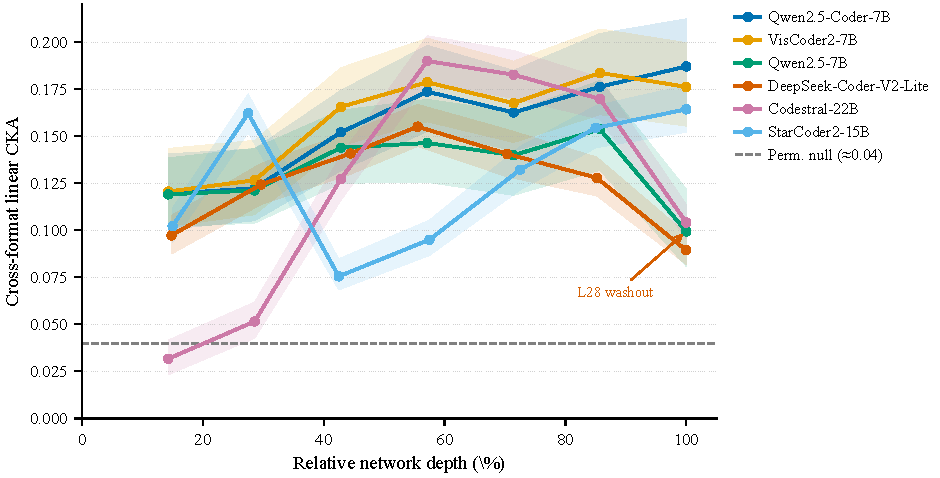
\includegraphics[width=\columnwidth]{figures/fig_cka_layer_curves_6model.pdf}
\caption{Bootstrap mean CKA (with 95\% CI shading) as a function of relative layer depth for six models across four architecture families. Colors encode profile type: inverted-U (Codestral, DeepSeek), bimodal (StarCoder2), broadly rising (Qwen2.5-Coder), and late-plateau (VisCoder2, Qwen2.5). The dashed grey line indicates the approximate permutation null (${\sim}0.04$).}
\label{fig:cka_layer_curves}
\end{figure}

\subsection{Negative Control: Non-Visual Code (C1)}
\label{sec:c1}

To test whether the cross-format signal is visual-specific, we conduct a pre-registered negative control (criterion D060, frozen before data collection).
We teacher-force 252 randomly sampled Python snippets through the three Qwen models and compute CKA between each Python--visual format pair (python--svg, python--tikz, python--asy) at all 7 layers (L4--L28), with 5{,}000 permutations for significance testing.
The design yields 3~models $\times$ 7~layers $\times$ 3~pairs = 63 python-X cells, directly comparable to the 63 visual-X cells (svg--tikz, svg--asy, tikz--asy) from the same experiment.

\paragraph{Magnitude (M1).}
The pre-registered criterion requires mean python-X CKA $< 0.5 \times$ mean visual-X CKA at each (model, layer) pair.
This criterion fails at 20 of 21 cells: python-X CKA ranges from 60--110\% of visual-X CKA across models and layers (Appendix Table~\ref{tab:c1_python_magnitude}).
The sole passing cell is Qwen2.5~base at L28 (python mean 0.030 vs.\ visual mean 0.076), driven by the sharp final-layer washout (F4) that depresses \emph{both} signals.
A second criterion (M2) further requires that permutation testing distinguish python from visual pairs (python $p > 0.05$ with visual $p < 0.001$), and a joint criterion (M3) requires $\geq 3$ models to satisfy both M1 and M2 at the same layer.

\paragraph{Early-layer homogeneity.}
At L4 and L8, all three models show python-X CKA within 80--120\% of visual-X CKA (anti-spin triggered), with python occasionally \emph{exceeding} visual (e.g., coder L4: ratio 1.06, qwen25 L4: 1.11).
Visual-X pairs at these layers also show weaker significance (L4: svg--tikz $p = 0.003$, failing the $p < 0.001$ threshold).
This early-layer convergence is consistent with the well-documented finding that lower transformer layers encode generic token-level features before task-specific structure emerges in deeper layers \cite{jawahar2019bert, tenney2019bert}.

\paragraph{Overall C1 verdict: FAIL.}
Per the pre-registered D060 criterion, C1 is declared FAIL: three independent fail modes are triggered (M1 magnitude at 20/21 cells; M3 joint criterion at 0/7 layers; anti-spin window at 6 cells in L4/L8).
The C1 result establishes that the measured cross-format CKA reflects code-general structure rather than visual-specific representations.

\paragraph{Scope: code-pretrained models only.}
An exploratory ablation with code-naive Llama-3-8B across 7 equidistant layers (Appendix~\ref{sec:llama-baseline}; D075, post-hoc) reveals that while visual cross-format CKA persists at comparable magnitude (21/21 cells $p < 0.005$), the python--visual entanglement does not arise (20/21 cells $p > 0.05$; the sole exception is python--Asy at L8 with borderline $p = 0.039$).
This indicates that the C1 failure mode---where python code yields 60--110\% of visual CKA---is specific to code-pretrained LLMs, not a general property of language models.

\subsection{Robustness Checks}
\label{sec:robustness}

\subsubsection{Procrustes Distance}
\label{sec:robustness-procrustes}

Orthogonal Procrustes distance (with PCA projection to $k=50$ dimensions) shows trends consistent with CKA across all models and layers.
Mean Procrustes values range from 0.094 to 0.158 (Table~\ref{tab:procrustes_mean}), with Qwen2.5 base at L28 again the lowest (0.094), confirming the layer-wise dynamics observed with CKA.

\begin{table}[!ht]
\centering
\small
\caption{Mean Procrustes distance (PCA $k$=50) per model at selected layers.}
\label{tab:procrustes_mean}
\resizebox{\columnwidth}{!}{%
\begin{tabular}{lccccc}
\toprule
Model & L4 & L12 & L16 & L24 & L28 \\
\midrule
Qwen2.5-Coder  & 0.102 & 0.138 & 0.158 & 0.157 & 0.153 \\
VisCoder2       & 0.102 & 0.142 & 0.157 & 0.158 & 0.146 \\
Qwen2.5 (base)  & 0.100 & 0.127 & 0.133 & 0.137 & 0.094 \\
\bottomrule
\end{tabular}}
\end{table}

\subsubsection{PWCCA (Auxiliary)}
\label{sec:robustness-pwcca}

PWCCA \cite{morcos2018pwcca} values (0.78--0.81 across all models) are directionally consistent with the CKA findings.
However, discriminative power is limited in the $n \ll d$ regime ($n{=}252$, $d$ up to $6{,}144$), where baseline canonical correlations are inflated, and we do not make significance claims based on PWCCA alone.
Procrustes distance, which does not suffer from this inflation, is a more reliable robustness check and shows trends fully consistent with CKA (\S\ref{sec:robustness-procrustes}).

\subsubsection{Token-Level Control}
\label{sec:robustness-token}

As an independent control analysis (computed over the full training corpora, not the probe pool), all three models share an identical Qwen2.5 tokenizer (151{,}643 vocabulary entries).
Pairwise token-ID Jaccard similarity between format corpora is uniformly low: SVG--TikZ = 0.025, SVG--Asy = 0.035, TikZ--Asy = 0.136.
The three-way token intersection covers only 1.2\% of the token union.
Format-exclusive tokens constitute $>$46\% of each format's active vocabulary.
This confirms that the 100\% format probe accuracy (\S\ref{sec:f1}) is a tokenization artifact: near-orthogonal token distributions allow perfect classification without relying on learned representations.

\subsubsection{Statistical Power}
\label{sec:robustness-power}

A1 power simulation (1{,}000 Monte Carlo iterations at layer L24) yields power = 1.0 for both $N{=}12$ (headline) and $N{=}18$ (auxiliary) configurations.
The observed CKA across all models (layer-averaged means: 0.123 for Coder, 0.124 for VisCoder2, 0.101 for base; Table~\ref{tab:a2_perm}) far exceeds the permutation null 95th percentile in every case.
This confirms that the permutation test has adequate power to detect CKA signals of the observed magnitude; it does not, however, confirm that the effect size is practically meaningful.


%% ============================================================
\FloatBarrier
\section{Discussion}
\label{sec:discussion}
%% ============================================================

The CKA signal ($2.55$--$3.01\times$ the permutation null across six models) is a second-order effect within representations overwhelmingly organized by format.
We cannot determine from CKA alone whether this reflects (a)~shared visual semantics, (b)~shared syntactic patterns, or (c)~artifacts of shared concept/prompt structure, and characterize it as \textbf{cross-format representational similarity of uncertain origin}.
The TikZ--Asy $\gg$ SVG--TikZ asymmetry (\S\ref{sec:f3}), which holds across all six models and four architecture families, tracks BPE token Jaccard at pair level ($\rho \approx 0.7$), establishing lexical overlap as a primary driver \cite{jawahar2019bert, hewitt-manning-2019-structural}.
The cell-level attenuation ($\rho = 0.57$) and layer-dependent CKA-to-Jaccard ratio growth indicate that tokenization alone does not fully account for the signal.
\label{sec:disc-syntax}
The pre-registered C1 negative control (\S\ref{sec:c1}) further constrains interpretation: python-X CKA reaches 60--110\% of visual-X CKA in magnitude, formally failing the D060 criterion at 20/21 (model, layer) cells.
This establishes that code-general structure---rather than visual-specific representations---dominates the measured alignment.

\paragraph{Split hypothesis (exploratory, D075).}
An ablation with code-naive Llama-3-8B across 7 equidistant layers (Appendix~\ref{sec:llama-baseline}) suggests a two-track interpretation:
(1)~visual cross-format CKA persists at comparable magnitude without code pretraining (21/21 cells $p < 0.005$), indicating that visual code formats share representational structure in general-purpose LLMs;
(2)~python--visual entanglement is substantially stronger in code-pretrained models: Qwen family python-X CKA reaches 60--110\% of visual-X magnitude (D060), whereas Llama-3-8B python-X cells are overwhelmingly non-significant (20/21 cells $p > 0.05$; sole exception: python--Asy L8, $p = 0.039$), suggesting that the C1 failure mode is a code-pretraining artifact.
We note that the 7-layer equidistant protocol samples to L28 (87.5\% depth), missing the final layers where the original three-layer scan (D075) found its only two significant python cells (L31, 97\% depth); python--visual entanglement in code-naive models, if present, may thus be confined to the deepest layers.
This observation is post-hoc and exploratory; confirmation requires pre-registered replication across additional code-naive architectures.

\paragraph{Methodological caveats.}
The fixed sample size ($n{=}252$ triples) constrains all models to the same statistical power, which may compress inter-model differences in CKA magnitude.
Additionally, the obs/null ratio ($2.55$--$3.01\times$) is more comparable across models than absolute CKA values, which vary with hidden dimensionality and model scale.

Key directions for resolving the origin ambiguity include: (1)~format-residualized CKA to project out the format-specific subspace; (2)~caption-conditioned partial correlation to isolate visual-specific signal; and (3)~visually-paired datasets where identical scenes are rendered in all three formats.


% Conclusion
% viscode_shared_subspace_probe — D028 framing
% Generated: 2026-04-11

\section{Conclusion}
\label{sec:conclusion}

We have presented a training-free probing framework for measuring cross-format representational similarity in visual code language models, combining linear CKA with bootstrap confidence intervals, permutation null testing, and Procrustes distance robustness check.

Applied to six models spanning four architecture families (Qwen, Mistral, BigCode, MoE) across SVG, TikZ, and Asymptote (252 matched triples, 7 equidistant layers per model), we find:
(i)~statistically significant but weak cross-format CKA in all six models ($2.55$--$3.01\times$ the permutation null, $p < 0.001$);
(ii)~a universal TikZ--Asy $\gg$ SVG--TikZ asymmetry consistent with a token-overlap gradient (BPE Jaccard $\rho \approx 0.7$ at pair level);
(iii)~architecture-dependent layer profiles---inverted-U, broadly rising, late-plateau, and bimodal---ruling out a universal ``mid-layer peak'' characterization; and
(iv)~a pre-registered non-visual Python negative control (D060) formally fails: python code yields 60--110\% of the visual CKA across 20/21 evaluation cells, establishing that code-general structure---rather than visual-specific representations---dominates the measured alignment.

The cross-format similarity is of \textbf{uncertain origin}: token-overlap gradient and code-general structure provide plausible non-visual explanations for the majority of the signal.
We release the complete analysis pipeline as a methodological template for future work on format-residualized CKA and visually-paired datasets to isolate genuine visual abstraction.


% ============================================================
% Limitations (ACL requires before references)
% ============================================================
% Limitations
% viscode_shared_subspace_probe — D028 framing
% Generated: 2026-04-11

\section{Limitations}
\label{sec:limitations}

\paragraph{(a) Sample size and model diversity.}
The headline Qwen analysis operates on $N{=}12$ cells, closer to a within-family ablation than a cross-model comparison.
The cross-architecture extension (\S\ref{sec:generalizability}) adds three models from distinct families (Mistral, BigCode, MoE), confirming that the weak signal generalizes.
However, all models are sampled at the same $n{=}252$ triples with 7 equidistant layers, which may compress inter-model differences.
Additional scales (e.g., 70B+), training paradigms (e.g., RLHF-heavy models), and non-Western tokenizers remain untested.

\paragraph{(b) Power interpretation.}
A1 power = 1.0 confirms that the permutation test can detect a CKA signal of the observed magnitude; it does \emph{not} establish that the effect size is large enough to be practically meaningful or to support claims about visual semantics.
The distinction between statistical significance and practical significance is critical given the small absolute CKA values (0.08--0.15).

\paragraph{(c) Contamination.}
VisCoder2 is fine-tuned on VisCode-Multi-679K, which includes VCM-Asy (overlapping with the probe pool source for Asymptote) and VCM-TikZ (71.7\% overlap with the TikZ probe pool source).
This creates a memorization floor for VisCoder2's Asy- and TikZ-related cells.
The headline $N{=}12$ statistic excludes VisCoder2 from the primary comparison as mitigation.
However, the remaining Qwen2.5 models may also have been exposed to SVG and TikZ content from Common Crawl during pretraining, a risk that cannot be fully quantified.

\paragraph{(d) No visual-level pairing.}
The probe pool is semantically matched via SBERT caption similarity (cosine $\geq 0.70$), not by rendering the same visual content in multiple formats.
True visual-level paired datasets---where identical geometric scenes are expressed in SVG, TikZ, and Asymptote---do not currently exist at sufficient scale.
Without such data, we cannot fully disentangle visual semantic similarity from textual and syntactic similarity in the CKA measurement.

\paragraph{(e) Scope of formats.}
We examine three visual code formats (SVG, TikZ, Asymptote), all of which produce 2D vector graphics.
The framework has not been tested on other visual code paradigms such as Processing, p5.js, or raster-generating code, nor on 3D formats.
The applicability of our findings to these broader settings is unknown.

\paragraph{(f) Negative control scope.}
Our pre-registered C1 negative control (\S\ref{sec:c1}) formally fails the D060 criterion: non-visual Python code yields 60--110\% of the visual cross-format CKA in magnitude across 3~models $\times$ 7~layers.
The Python snippets are randomly sampled (not semantically matched to the visual triples), which limits the precision of this comparison.
A stronger control would use semantically matched non-visual code triples (e.g., Python programs describing analogous computational structures), which remains a non-trivial dataset construction challenge.
This failure establishes that the measured cross-format signal reflects code-general rather than visual-specific structure; the random sampling limits only the precision of this quantification, not the qualitative conclusion.


% ============================================================
% References
% ============================================================
\bibliography{references}

% ============================================================
% Appendix (complete numerical tables)
% ============================================================
\appendix
% appendix.tex — Complete numerical tables for the cross-format probing study
\section*{Appendix}
\label{sec:appendix}

\setcounter{table}{0}
\renewcommand{\thetable}{A\arabic{table}}

%% ========================================================================
%% Table A1: Complete CKA Values
%% ========================================================================
\begin{table*}[t]
\centering
\caption{Complete CKA similarity values per model, layer, and format pair. Mean is the arithmetic average of the three format pairs, consistent with main text Table~\ref{tab:cka_mean}.}
\label{tab:cka_complete}
\small
\begin{tabular}{ll rrrr}
\toprule
\textbf{Model} & \textbf{Layer} & \textbf{SVG--TikZ} & \textbf{SVG--Asy} & \textbf{TikZ--Asy} & \textbf{Mean} \\
\midrule
Qwen2.5-Coder & L4  & 0.049 & 0.092 & 0.120 & 0.087 \\
Qwen2.5-Coder & L8  & 0.059 & 0.087 & 0.125 & 0.090 \\
Qwen2.5-Coder & L12 & 0.067 & 0.098 & 0.200 & 0.121 \\
Qwen2.5-Coder & L16 & 0.086 & 0.124 & 0.212 & 0.141 \\
Qwen2.5-Coder & L20 & 0.087 & 0.118 & 0.180 & 0.128 \\
Qwen2.5-Coder & L24 & 0.105 & 0.109 & 0.209 & 0.141 \\
Qwen2.5-Coder & L28 & 0.103 & 0.114 & 0.229 & 0.149 \\
\midrule
VisCoder2      & L4  & 0.050 & 0.092 & 0.122 & 0.088 \\
VisCoder2      & L8  & 0.062 & 0.089 & 0.133 & 0.095 \\
VisCoder2      & L12 & 0.075 & 0.103 & 0.218 & 0.132 \\
VisCoder2      & L16 & 0.089 & 0.124 & 0.216 & 0.143 \\
VisCoder2      & L20 & 0.086 & 0.124 & 0.181 & 0.130 \\
VisCoder2      & L24 & 0.102 & 0.125 & 0.208 & 0.145 \\
VisCoder2      & L28 & 0.093 & 0.116 & 0.203 & 0.137 \\
\midrule
Qwen2.5-Base   & L4  & 0.050 & 0.087 & 0.118 & 0.085 \\
Qwen2.5-Base   & L8  & 0.058 & 0.087 & 0.122 & 0.089 \\
Qwen2.5-Base   & L12 & 0.061 & 0.093 & 0.182 & 0.112 \\
Qwen2.5-Base   & L16 & 0.067 & 0.112 & 0.166 & 0.115 \\
Qwen2.5-Base   & L20 & 0.070 & 0.104 & 0.153 & 0.109 \\
Qwen2.5-Base   & L24 & 0.086 & 0.099 & 0.177 & 0.121 \\
Qwen2.5-Base   & L28 & 0.044 & 0.081 & 0.104 & 0.076 \\
\bottomrule
\end{tabular}
\end{table*}

%% ========================================================================
%% Table A2: Procrustes Distance
%% ========================================================================
\begin{table*}[t]
\centering
\caption{Procrustes distance per model, layer, and format pair.  Lower values indicate greater representational similarity after optimal rotation.}
\label{tab:procrustes_complete}
\small
\begin{tabular}{ll rrr r}
\toprule
\textbf{Model} & \textbf{Layer} & \textbf{SVG--TikZ} & \textbf{SVG--Asy} & \textbf{TikZ--Asy} & \textbf{Mean} \\
\midrule
Qwen2.5-Coder & L4  & 0.073 & 0.095 & 0.139 & 0.102 \\
Qwen2.5-Coder & L8  & 0.079 & 0.095 & 0.146 & 0.107 \\
Qwen2.5-Coder & L12 & 0.090 & 0.106 & 0.217 & 0.138 \\
Qwen2.5-Coder & L16 & 0.113 & 0.134 & 0.226 & 0.158 \\
Qwen2.5-Coder & L20 & 0.113 & 0.128 & 0.198 & 0.146 \\
Qwen2.5-Coder & L24 & 0.124 & 0.128 & 0.219 & 0.157 \\
Qwen2.5-Coder & L28 & 0.117 & 0.124 & 0.220 & 0.153 \\
\midrule
VisCoder2      & L4  & 0.072 & 0.094 & 0.141 & 0.102 \\
VisCoder2      & L8  & 0.080 & 0.095 & 0.150 & 0.108 \\
VisCoder2      & L12 & 0.095 & 0.108 & 0.222 & 0.142 \\
VisCoder2      & L16 & 0.115 & 0.133 & 0.222 & 0.157 \\
VisCoder2      & L20 & 0.115 & 0.133 & 0.195 & 0.148 \\
VisCoder2      & L24 & 0.123 & 0.136 & 0.216 & 0.158 \\
VisCoder2      & L28 & 0.110 & 0.125 & 0.202 & 0.146 \\
\midrule
Qwen2.5-Base   & L4  & 0.071 & 0.093 & 0.136 & 0.100 \\
Qwen2.5-Base   & L8  & 0.077 & 0.091 & 0.141 & 0.103 \\
Qwen2.5-Base   & L12 & 0.083 & 0.097 & 0.201 & 0.127 \\
Qwen2.5-Base   & L16 & 0.093 & 0.113 & 0.193 & 0.133 \\
Qwen2.5-Base   & L20 & 0.096 & 0.112 & 0.177 & 0.128 \\
Qwen2.5-Base   & L24 & 0.104 & 0.112 & 0.195 & 0.137 \\
Qwen2.5-Base   & L28 & 0.065 & 0.084 & 0.133 & 0.094 \\
\bottomrule
\end{tabular}
\end{table*}

%% ========================================================================
%% Table A3: PWCCA Values
%% ========================================================================
\begin{table*}[t]
\centering
\caption{Projection-Weighted CCA (PWCCA; \citealt{morcos2018pwcca}) mean similarity per model and layer.  Higher values indicate stronger cross-format alignment.}
\label{tab:pwcca_complete}
\small
\begin{tabular}{ll r}
\toprule
\textbf{Model} & \textbf{Layer} & \textbf{PWCCA} \\
\midrule
Qwen2.5-Coder & L4  & 0.7699 \\
Qwen2.5-Coder & L8  & 0.7734 \\
Qwen2.5-Coder & L12 & 0.8128 \\
Qwen2.5-Coder & L16 & 0.8194 \\
Qwen2.5-Coder & L20 & 0.7989 \\
Qwen2.5-Coder & L24 & 0.7786 \\
Qwen2.5-Coder & L28 & 0.7791 \\
\midrule
VisCoder2      & L4  & 0.7680 \\
VisCoder2      & L8  & 0.7743 \\
VisCoder2      & L12 & 0.8046 \\
VisCoder2      & L16 & 0.8086 \\
VisCoder2      & L20 & 0.7885 \\
VisCoder2      & L24 & 0.7764 \\
VisCoder2      & L28 & 0.7712 \\
\midrule
Qwen2.5-Base   & L4  & 0.7587 \\
Qwen2.5-Base   & L8  & 0.7657 \\
Qwen2.5-Base   & L12 & 0.8012 \\
Qwen2.5-Base   & L16 & 0.8068 \\
Qwen2.5-Base   & L20 & 0.7932 \\
Qwen2.5-Base   & L24 & 0.7760 \\
Qwen2.5-Base   & L28 & 0.8114 \\
\bottomrule
\end{tabular}
\end{table*}

%% ========================================================================
%% Table A4: Permuted-Label Probe Results
%% ========================================================================
\begin{table*}[t]
\centering
\caption{Format-classification probe accuracy with real vs.\ permuted labels.  The large gap ($\approx 0.667$) confirms that probe accuracy reflects genuine format information rather than memorized structure.}
\label{tab:permuted_probe}
\small
\begin{tabular}{ll rrr}
\toprule
\textbf{Model} & \textbf{Layer} & \textbf{Real Acc.} & \textbf{Permuted Acc.} & \textbf{Gap} \\
\midrule
Qwen2.5-Coder & L4  & 1.000 & 0.333 & 0.667 \\
Qwen2.5-Coder & L8  & 1.000 & 0.333 & 0.667 \\
Qwen2.5-Coder & L12 & 1.000 & 0.333 & 0.667 \\
Qwen2.5-Coder & L16 & 1.000 & 0.333 & 0.667 \\
Qwen2.5-Coder & L20 & 1.000 & 0.333 & 0.667 \\
Qwen2.5-Coder & L24 & 1.000 & 0.333 & 0.667 \\
Qwen2.5-Coder & L28 & 1.000 & 0.333 & 0.667 \\
\midrule
VisCoder2      & L4  & 1.000 & 0.333 & 0.667 \\
VisCoder2      & L8  & 1.000 & 0.333 & 0.667 \\
VisCoder2      & L12 & 1.000 & 0.333 & 0.667 \\
VisCoder2      & L16 & 1.000 & 0.333 & 0.667 \\
VisCoder2      & L20 & 1.000 & 0.333 & 0.667 \\
VisCoder2      & L24 & 1.000 & 0.333 & 0.667 \\
VisCoder2      & L28 & 1.000 & 0.333 & 0.667 \\
\midrule
Qwen2.5-Base   & L4  & 1.000 & 0.333 & 0.667 \\
Qwen2.5-Base   & L8  & 1.000 & 0.333 & 0.667 \\
Qwen2.5-Base   & L12 & 1.000 & 0.333 & 0.667 \\
Qwen2.5-Base   & L16 & 1.000 & 0.333 & 0.667 \\
Qwen2.5-Base   & L20 & 1.000 & 0.333 & 0.667 \\
Qwen2.5-Base   & L24 & 1.000 & 0.333 & 0.667 \\
Qwen2.5-Base   & L28 & 1.000 & 0.333 & 0.667 \\
\bottomrule
\end{tabular}
\end{table*}

%% ========================================================================
%% Table A5: A2 Permutation Test Summary
%% ========================================================================
\begin{table*}[t]
\centering
\caption{A2 permutation test ($n{=}5{,}000$): observed cross-format CKA mean vs.\ null distribution obtained by permuting sample identities within each format.  $p{<}0.001$ for all models confirms that cross-format representational similarity is not an artifact of format-level statistics.}
\label{tab:a2_permutation}
\small
\begin{tabular}{l rrrr}
\toprule
\textbf{Model} & \textbf{Obs.\ CKA Mean} & \textbf{Null Mean} & \textbf{Null Std} & \textbf{$p$-value} \\
\midrule
Qwen2.5-Coder & 0.123 & 0.041 & 0.003 & ${<}\,0.001$ \\
VisCoder2      & 0.124 & 0.044 & 0.003 & ${<}\,0.001$ \\
Qwen2.5-Base   & 0.101 & 0.037 & 0.003 & ${<}\,0.001$ \\
\bottomrule
\end{tabular}
\end{table*}

%% ========================================================================
%% Algorithm: Permutation Test Pseudocode
%% ========================================================================

\begin{algorithm}[h!]
\caption{A2 Permutation Null Test for Cross-Format CKA}
\label{alg:perm_test}
\begin{algorithmic}[1]
\REQUIRE Hidden-state matrices $\mathbf{H}^{(m,f,l)} \in \mathbb{R}^{N \times d}$ for model $m$, format $f$, layer $l$
\REQUIRE Number of permutations $B = 5{,}000$
\STATE \textbf{H$_0$:} Cross-format CKA arises solely from format-level statistics; sample identity carries no aligned signal across formats.
\FOR{each model $m$}
  \STATE Compute observed CKA for each $(l, f_1, f_2)$ pair from aligned Gram matrices
  \STATE $\bar{c}_\text{obs} \leftarrow \text{mean over all layers and pairs}$
  \FOR{$b = 1$ to $B$}
    \STATE Draw random permutation $\pi$ of $\{1, \ldots, N\}$
    \FOR{each layer $l$ and pair $(f_1, f_2)$}
      \STATE Permute rows and columns of $\mathbf{K}^{(f_2)}$ by $\pi$: $\tilde{\mathbf{K}}^{(f_2)}_{ij} = \mathbf{K}^{(f_2)}_{\pi(i),\pi(j)}$
      \STATE Compute $\text{CKA}(\mathbf{K}^{(f_1)}, \tilde{\mathbf{K}}^{(f_2)})$
    \ENDFOR
    \STATE $\bar{c}_\text{null}^{(b)} \leftarrow \text{mean over all layers and pairs}$
  \ENDFOR
  \STATE $p \leftarrow \frac{1}{B} \sum_{b=1}^{B} \mathbf{1}[\bar{c}_\text{null}^{(b)} \geq \bar{c}_\text{obs}]$
\ENDFOR
\ENSURE Per-model $p$-value, null distribution $\{\bar{c}_\text{null}^{(b)}\}_{b=1}^B$, observed/null ratio
\end{algorithmic}
\end{algorithm}

%% ========================================================================
%% Table A6: Format Probe Accuracy (moved from main text)
%% ========================================================================
\begin{table}[h!]
\centering
\small
\caption{Format classification probe accuracy (5-fold CV, logistic regression). All 21 model--layer cells are 1.0000.}
\label{tab:probe_accuracy}
\resizebox{\columnwidth}{!}{%
\begin{tabular}{lccccccc}
\toprule
Model & L4 & L8 & L12 & L16 & L20 & L24 & L28 \\
\midrule
Qwen2.5-Coder  & 1.0000 & 1.0000 & 1.0000 & 1.0000 & 1.0000 & 1.0000 & 1.0000 \\
VisCoder2       & 1.0000 & 1.0000 & 1.0000 & 1.0000 & 1.0000 & 1.0000 & 1.0000 \\
Qwen2.5-Base    & 1.0000 & 1.0000 & 1.0000 & 1.0000 & 1.0000 & 1.0000 & 1.0000 \\
\bottomrule
\end{tabular}}
\end{table}

%% ========================================================================
%% Table A7: PWCCA Null Calibration (moved from main text)
%% ========================================================================
\begin{table}[h!]
\centering
\small
\caption{PWCCA permutation null calibration (300 perms). The observed/null gap is statistically significant but small (ratio ${\sim}1.1\times$), compared to CKA's ${\sim}3\times$ null ratio.}
\label{tab:pwcca_null}
\resizebox{\columnwidth}{!}{%
\begin{tabular}{lcccc}
\toprule
Model & Observed & Null (mean$\pm$std) & Ratio & $p$ \\
\midrule
Qwen2.5-Coder  & 0.790 & 0.688$\pm$0.004 & 1.148$\times$ & $<$0.001 \\
VisCoder2       & 0.785 & 0.685$\pm$0.004 & 1.145$\times$ & $<$0.001 \\
Qwen2.5-Base    & 0.788 & 0.699$\pm$0.004 & 1.127$\times$ & $<$0.001 \\
\bottomrule
\end{tabular}}
\end{table}

%% ========================================================================
%% Table A8: SBERT Threshold Sensitivity (C3)
%% ========================================================================
\begin{table}[h!]
\centering
\small
\caption{SBERT threshold sensitivity (C3): mean CKA at L28 by matching threshold. All 252 triples have min cosine $\geq 0.70$, so thresholds $\leq 0.70$ yield identical pools. At thresholds $\geq 0.75$, $N$ drops sharply, making CKA estimates unreliable due to $n \ll d$ inflation \cite{nguyen2021wide}; we do not interpret these values as evidence of stronger alignment. The relative ordering TikZ--Asy $>$ SVG--Asy $>$ SVG--TikZ is preserved at $N{=}51$, consistent with the token-overlap gradient (F3).}
\label{tab:sbert_sensitivity}
\begin{tabular}{rr ccc}
\toprule
Threshold & $N$ & Coder & VisCoder2 & Base \\
\midrule
0.60 & 252 & 0.149 & 0.137 & 0.076 \\
0.65 & 252 & 0.149 & 0.137 & 0.076 \\
0.70 & 252 & 0.149 & 0.137 & 0.076 \\
0.75 &  51 & 0.252 & 0.247 & 0.146 \\
0.80 &   6 & 0.739 & 0.766 & 0.616 \\
\bottomrule
\end{tabular}
\end{table}

%% ========================================================================
%% Stage A Generation Details (moved from Methods for space)
%% ========================================================================
\paragraph{Stage A generation details.}
Eval pool sources: SVG from VisPlotBench and VCM-SVG; TikZ from DaTikZ v1 test; Asymptote from VisPlotBench and VCM-Asy.
All sources filtered uniformly: code length $\in [50, 8000]$ characters, caption length $\in [10, 3000]$ characters, render success within 30s, normalized-code-hash deduplication.
Generation uses vLLM \cite{vllm} in fp16 with $T{=}0.3$, $\text{top\_p}{=}1.0$, $n{=}1$, format-specific max tokens (SVG/TikZ: 1024, Asy: 2048).
3-shot exemplars are drawn from independent training data disjoint from both eval and probe pools.
The CLIPScore SNR gate was calibrated in a pilot study ($n{=}20$, 5 dimensions) using a shuffle-permutation null.

%% ========================================================================
%% Table A9: Stage A Generation Summary
%% ========================================================================
\begin{table}[h!]
\centering
\small
\caption{Stage A generation summary: validity rate per model and format (3,600 total, 0-shot and 3-shot pooled). Temperature $T{=}0.3$, $n{=}1$ per prompt. (Table~A9)}
\label{tab:stage_a_summary}
\resizebox{\columnwidth}{!}{%
\begin{tabular}{lccc}
\toprule
Model & SVG & TikZ & Asy \\
\midrule
Qwen2.5-Coder  & 1.000 & 0.995 & 1.000 \\
VisCoder2       & 0.972 & 0.962 & 1.000 \\
Qwen2.5-Base    & 0.662 & 0.722 & 0.752 \\
\midrule
Overall         & \multicolumn{3}{c}{3,227/3,600 valid (89.6\%)} \\
\bottomrule
\end{tabular}}
\end{table}

\paragraph{PWCCA in the $n \ll d$ regime.}
The limited discriminative power of PWCCA in this study reflects known properties of CCA when sample size is much smaller than feature dimensionality.
With $n{=}252$ samples and $d{=}3{,}584$ features (ratio 0.07), canonical correlations converge toward 1.0 regardless of true signal strength, compressing the dynamic range available to distinguish signal from noise.
This is the same degeneracy that motivated our removal of raw CCA from the analysis pipeline.
PWCCA corroborates the \emph{direction} of the CKA signal---observed values exceed the permutation null for all three models---but its observed/null ratio (1.13--1.15$\times$) is far below CKA's (${\sim}3\times$), limiting its value as an independent robustness check in this experimental design.

%% ========================================================================
%% C1 Negative Control: Python-X vs Visual-X Magnitude
%% ========================================================================

\subsection{C1 Negative Control: Python-X vs.\ Visual-X Magnitude}
\label{sec:c1-magnitude}

Table~\ref{tab:c1_python_magnitude} reports the per-cell comparison underlying the C1 pre-registered criterion (D060): mean python-X CKA must be $< 0.5\times$ mean visual-X CKA at each (model, layer) cell.
The criterion fails at 20 of 21 cells; only Qwen2.5-base at L28 passes, driven by the sharp final-layer washout (F4) that depresses both signals.

\begin{table}[!ht]
\centering
\small
\caption{C1 negative control magnitude comparison. Python-X = mean CKA across (python--svg, python--tikz, python--asy); Visual-X = mean CKA across (svg--tikz, svg--asy, tikz--asy). Ratio = Python-X\,/\,Visual-X. M1 criterion requires Ratio $< 0.50$; \textbf{bold} = the sole passing cell. \emph{Note:} $p$-values report the minimum across three format pairs per cell (uncorrected for multiplicity).}
\label{tab:c1_python_magnitude}
\begin{tabular}{llccccc}
\toprule
Model & Layer & Py-X CKA & Vis-X CKA & Ratio & Min $p$ (Py, uncorr.) & M1 \\
\midrule
Coder-7B & L4  & 0.093 & 0.087 & 1.06 & .015 & \ding{55} \\
Coder-7B & L8  & 0.088 & 0.091 & 0.98 & .056 & \ding{55} \\
Coder-7B & L12 & 0.092 & 0.121 & 0.76 & .033 & \ding{55} \\
Coder-7B & L16 & 0.089 & 0.141 & 0.63 & .064 & \ding{55} \\
Coder-7B & L20 & 0.084 & 0.128 & 0.65 & .198 & \ding{55} \\
Coder-7B & L24 & 0.092 & 0.141 & 0.65 & .079 & \ding{55} \\
Coder-7B & L28 & 0.102 & 0.149 & 0.69 & .005 & \ding{55} \\
\midrule
VisCoder2-7B & L4  & 0.093 & 0.088 & 1.05 & .026 & \ding{55} \\
VisCoder2-7B & L8  & 0.091 & 0.095 & 0.97 & .048 & \ding{55} \\
VisCoder2-7B & L12 & 0.099 & 0.132 & 0.75 & .047 & \ding{55} \\
VisCoder2-7B & L16 & 0.096 & 0.143 & 0.67 & .049 & \ding{55} \\
VisCoder2-7B & L20 & 0.086 & 0.130 & 0.66 & .182 & \ding{55} \\
VisCoder2-7B & L24 & 0.087 & 0.145 & 0.60 & .065 & \ding{55} \\
VisCoder2-7B & L28 & 0.091 & 0.137 & 0.66 & .023 & \ding{55} \\
\midrule
Qwen2.5-base & L4  & 0.094 & 0.085 & 1.11 & .047 & \ding{55} \\
Qwen2.5-base & L8  & 0.087 & 0.089 & 0.98 & .103 & \ding{55} \\
Qwen2.5-base & L12 & 0.088 & 0.112 & 0.78 & .110 & \ding{55} \\
Qwen2.5-base & L16 & 0.079 & 0.115 & 0.68 & .127 & \ding{55} \\
Qwen2.5-base & L20 & 0.071 & 0.109 & 0.65 & .319 & \ding{55} \\
Qwen2.5-base & L24 & 0.075 & 0.121 & 0.62 & .242 & \ding{55} \\
Qwen2.5-base & L28 & \textbf{0.030} & \textbf{0.076} & \textbf{0.39} & .236 & \textbf{\ding{51}} \\
\bottomrule
\end{tabular}
\end{table}

\paragraph{Multiplicity note.}
The 9/21 significant cells reported above use per-pair permutation $p$-values without multiplicity correction across the three format pairs tested at each (model, layer) cell.
Under Bonferroni correction for three comparisons per cell ($\alpha = 0.0167$), the Qwen family retains 2/21 significant python-X cells (Coder L4 $p{=}.015$ and L28 $p{=}.005$) versus Llama-3-8B 0/21.
The qualitative split in detectability therefore holds under correction, though the effect size shrinks from 9/21 to 2/21.

%% ========================================================================
%% Code-Naive Baseline: Llama-3-8B
%% ========================================================================

\subsection{Code-Naive Baseline: Llama-3-8B}
\label{sec:llama-baseline}

\paragraph{Note:} The initial three-layer scan was exploratory (D075); a subsequent 7-layer test with pre-registered criteria (D078: visual $\geq$70\% \& python $\leq$40\% significance) confirmed the pattern.

To test whether the cross-format CKA signal requires code-specialized pretraining, we apply the same probing framework to Meta-Llama-3-8B (base), a general-purpose LLM with no code-specific training.
We extract hidden states at 7 equidistant layers (L4/L8/L12/L16/L20/L24/L28 out of 32, corresponding to 12.5--87.5\% depth) for all 252 triples and 252 Python snippets, computing CKA with 5{,}000 permutations and 1{,}000 bootstrap subsamples.

\begin{table}[!ht]
\centering
\small
\caption{Llama-3-8B baseline CKA across 7 equidistant layers: visual cross-format pairs (top) and python--visual pairs (bottom). Bold $p$-values indicate $p < 0.005$. \emph{Note:} $p$-values are per-pair permutation tests (5{,}000 permutations, uncorrected).}
\label{tab:llama_baseline}
\begin{tabular}{lccccccc}
\toprule
Pair & L4 & L8 & L12 & L16 & L20 & L24 & L28 \\
\midrule
\multicolumn{8}{l}{\emph{Visual cross-format pairs (21/21 significant, all $p < 0.005$)}} \\
SVG--TikZ   & .053 & .071 & .078 & .090 & .092 & .089 & .088 \\
SVG--Asy    & .075 & .082 & .087 & .103 & .093 & .089 & .093 \\
TikZ--Asy   & .126 & .181 & .189 & .208 & .191 & .183 & .174 \\
\midrule
\multicolumn{8}{l}{\emph{Python--visual pairs (1/21 significant: Py--Asy L8, $p{=}.039$)}} \\
Py--SVG  & .060 & .059 & .061 & .069 & .059 & .051 & .054 \\
         & \scriptsize{.184} & \scriptsize{.517} & \scriptsize{.446} & \scriptsize{.435} & \scriptsize{.644} & \scriptsize{.652} & \scriptsize{.701} \\
Py--TikZ & .085 & .098 & .103 & .102 & .094 & .084 & .087 \\
         & \scriptsize{.182} & \scriptsize{.151} & \scriptsize{.160} & \scriptsize{.189} & \scriptsize{.130} & \scriptsize{.119} & \scriptsize{.096} \\
Py--Asy  & .107 & .115 & .116 & .118 & .092 & .083 & .093 \\
         & \scriptsize{.118} & \scriptsize{\textbf{.039}} & \scriptsize{.146} & \scriptsize{.221} & \scriptsize{.310} & \scriptsize{.218} & \scriptsize{.127} \\
\bottomrule
\end{tabular}
\end{table}

Visual cross-format CKA is significant at all 21 cells ($p \leq 0.0024$; mean 0.116).
The TikZ--Asy $>$ SVG--Asy $>$ SVG--TikZ ordering replicates at all 7 layers, strengthening the token-overlap gradient (F3) as robust to the absence of code-specialized pretraining.
In contrast, python--visual pairs are overwhelmingly non-significant (20/21 cells $p > 0.05$); the sole exception is Python--Asy at L8 ($p = 0.039$), a borderline result that does not survive multiplicity correction.

We note that the equidistant protocol samples Llama-3 to L28 (87.5\% depth), missing the final layer (L31, 97\% depth) where D075's three-layer scan found the only two significant python cells.
Thus, python--visual entanglement in code-naive Llama-3, if present, is \emph{layer-local} (present only at the deepest tested layer in D075, L31, 97\% depth), whereas in code-pretrained Qwen models, python-X significance is broader (9/21 cells $p<0.05$, uncorrected) with observed-to-null ratios of ${\sim}1.3$--$1.7\times$ versus Llama's $0.95$--$1.09\times$.
Importantly, the magnitude pattern is shared: Llama's python/visual CKA ratios (0.60--0.99) overlap with the Qwen range (0.60--1.11).
The split is thus in \emph{permutation detectability}---code pretraining elevates python-X CKA above the permutation null---not in raw magnitude.


\end{document}
